\documentclass[10pt,a4paper]{scrartcl}
\usepackage[utf8]{inputenc}
\usepackage{polski}
\usepackage[polish]{babel}
\usepackage{amsmath}
\usepackage{enumitem}
\usepackage{graphicx}
\usepackage{float}
\usepackage{geometry}
\usepackage{makecell}
\usepackage{listings,xcolor}
\usepackage{gensymb}
\geometry{left=2.5cm,right=2.5cm,top=2.5cm,bottom=2.5cm}
\restylefloat{table}
\author{Konrad Maciałek}
\title{Telemetria pojazdów mechanicznych}
\subtitle{Projekt Zespołowy}
\lstset{
	string=[s]{"}{"},
	stringstyle=\color{blue},
	comment=[l]{:},
	commentstyle=\color{black},
}
\begin{document}
	\pagenumbering{gobble}
	\maketitle
	\newpage
	\pagenumbering{arabic}
	\section{Zadanie projektowe}
	Zaprojektowanie rozwiązania, służącego do zdalnej diagnostyki pojazdów samochodowych. Powstałe urządzenie wraz z aplikacją powinno umożliwiać analizę danych, odczytanych z podstawowych czujników wbudowanych we współczesne samochody.
	\\
	Dane powinny być dostępne poprzez stronę www.
	\section{Opis projektu}
		\subsection{Ogólny opis rozwiązania problemu}
		\begin{figure}[H]
			\centering
			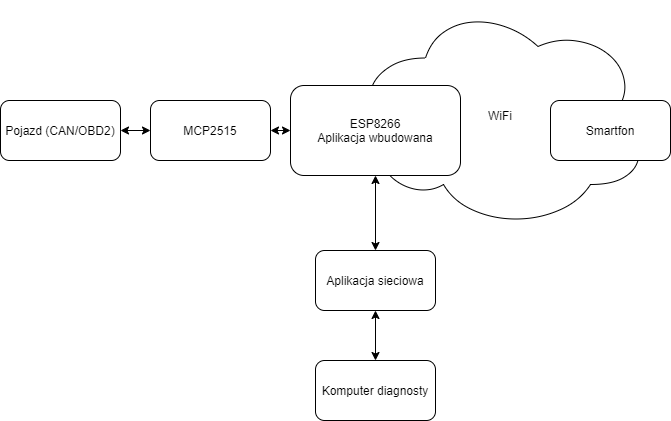
\includegraphics[width=0.7\linewidth]{./remoteCarDiagz.drawio}
			\caption[Diagram ogólny]{Diagram ogólny}
			\label{fig:remotecardiagz}
		\end{figure}
		Finałowy produkt składa się z dwóch głównych części: sprzętowej, odczytującej zadane dane oraz drugiej- aplikacji sieciowej, umożliwiającej podgląd i sterowanie danymi. 
		\subsubsection{Odczyt danych (VagCan)}
		Głównym elementem sterującym jest mikro-kontroler ESP8266. Działająca w nim aplikacja komunikuje się z systemami diagnostyki OBD pojazdu za pomocą protokołu CAN poprzez kontroler MCP2515. Pobrane informacje wysyła następnie poprzez sieć WiFi udostępnioną ze telefonu, do aplikacji sieciowej, gdzie są one zapisywane i udostępniane użytkownikowi końcowemu. 
		\subsubsection{Aplikacja sieciowa (RemoteCarDiagz)}
		Aplikacja sieciowa składa się z kilku komponentów: serwisu aplikacyjnego typu REST API, publikującego interfejs umożliwiający odczyt i zapis danych oraz aplikacji klienckiej z graficznym interfejsem użytkownika, pozwalającym na podgląd oraz manipulację danymi. Dodatkowo wykorzystano serwisy wspomagające, takie jak baza danych Prometheus, zoptymalizowana do zapisu i odczytu danych zaszeregowanych czasowo.
		
		\subsection{Wybór technologii}
		Wszystkie technologie zostały wybrane mając na uwadze ograniczenia licencyjne, tj. narzędzia, biblioteki, środowiska programistyczne są oparte na otwartym kodzie, przy wykorzystaniu licencji GPL lub podobnych. Cały projekt został stworzony pod kontrolą systemu operacyjnego Linux/Ubuntu.
			\subsubsection{Część odczytująca dane}
			Wybór mikrokontrolera ESP8266 podyktowany został łatwością implementacji obsługi transmisji danych w sieci WiFi.  MCP2515 jest natomiast najpopularniejszym kontrolerem służącym do obsługi magistrali CAN.  
			Z uwagi na powyższe, oraz dostępność bibliotek programistycznych, wybór technologii został ograniczony środowiskiem- język C++ pod kontrolą Visual Studio Code.
			\subsubsection{Aplikacja sieciowa}
			Z uwagi na wcześniejsze doświadczenie w języku C\# oraz chęć poznania nowych technologii, zdecydowano się na wybór .Net5. Wybór ten pozwolił na zaimplementowanie aplikacji klienckiej przy wykorzystaniu nowoczesnego frameworka Blazor WASM.
	
		\subsection{Protokół OBD i CAN}
		On-board diagnostics (OBD) jest terminem opisującym systemy autodiagnostyki pojazdów samochodowych. Po raz pierwszy został wprowadzony w latach 80. XX wieku w Stanach Zjednoczonych, mając na celu umożliwienie szybkiej detekcji nieprawidłowości związanych z emisją zanieczyszczeń do atmosfery.  Nowoczesne implementacje dają możliwość wglądu do danych diagnostycznych zbieranych przez elektroniczne moduły kontroli (ECU) zainstalowane w pojazdach mechanicznych, poprzez standaryzowane złącze OBD-II:
		\begin{figure}[H]
			\centering
			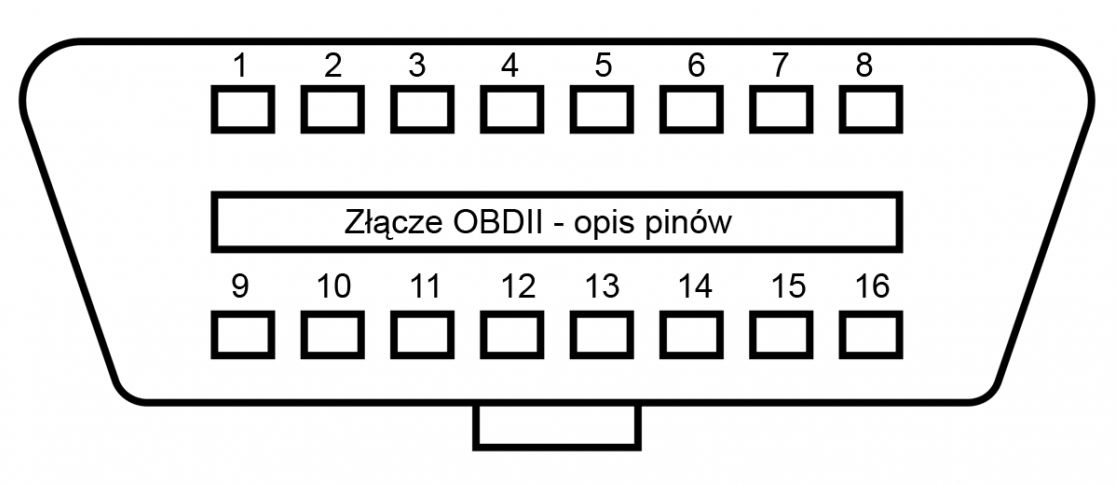
\includegraphics[width=0.7\linewidth]{obd2}
			\caption[Złącze OBD-II]{Złącze OBD-II- opis pinów}
			\label{fig:obd2}
		\end{figure}
		\begin{table}[H]
		\begin{tabular}{|c|c|}
			\hline
			Pin & Opis \\
			\hline
			4 & masa \\
			\hline
			16 & +12V z akumulatora \\
				\hline
			6 & CAN High \\			
				\hline
			14 & CAN Low \\			
			\hline
		\end{tabular}
		\end{table}
		
		Na powyższym diagramie opisano tylko piny wykorzystane w projekcie, z czego najważniejszymi są 6 i 14. Są to piny umożliwiające komunikację poprzez protokół magistrali CAN (sformułowany w normach ISO 15765-4 i SAE J2284).\\
		CAN to szeregowa magistrala komunikacyjna, mająca głównie zastosowanie w przemyśle samochodowym, powstała w latach 80. XX wieku. Wykorzystuje ona dwuprzewodową skrętkę, co pozwala uzyskać prędkość przesyłu na poziomie 1MB/s przy dystansie do 40 metrów. Z uwagi na brak jednostki nadrzędnej, komunikacja ma charakter rozgłoszeniowy, tzn. komunikaty nadawane na magistralę, odbierane są przez wszystkie urządzenia do niej podpięte. W przypadku pojazdu samochodowego, urządzeniami używającymi tej magistrali są ECU, odpowiedzialne np. za działanie silnika lub systemów bezpieczeństwa, takich jak ABS.\\ \\ Najważniejsze cechy:
		\begin{itemize}
			\item 8 bitów danych w komunikacie
			\item rozpoznawanie komunikatów poprzez identyfikatory
			\item automatyczna obsługa dostępu do magistrali
			\item sprzętowa obsługa błędów
		\end{itemize}
		
		\subsubsection{PID}
		W standardzie OBD-II poszczególne parametry diagnostyczne dostępne są poprzez identyfikatory PID (parameter identification number). Żądanie wysyłane za pomocą linii CAN zawiera identyfikator PID, co pozwala odpowiednim modułom pojazdu na nie odpowiedzieć. Przykładowe parametry podano w tabeli poniżej. \\\\
		\begin{tabular}{|l|l|}
			\hline
			PID & Opis \\
			\hline
			0x03 & Status układu paliwowego \\
			\hline
			0x04 & Obliczone obciążenie silnika \\
			\hline
			0x05 & Temperatura czynnika chłodzącego\\			
			\hline
			0x0 & Aktualna prędkość samochodu \\			
			\hline
		\end{tabular}
		\\\\
		Norma SAE J1979 definiuje również 10 serwisów, grupujących dane. W projekcie wykorzystano tylko serwis 01, podający aktualne dane diagnostyczne. Przykładowo, serwis 02 podaje te same dane, ale zebrane podczas ostatniego wystąpienia błędu diagnostycznego.
		\subsubsection{Format komunikacji}
		Czytnik diagnostyczny rozpoczyna komunikację poprzez wysłanie żądania pod adres 0x7DFh, który pełni funkcję adresu rozgłoszeniowego. ECU, które potrafią odpowiedzieć na żądania OBD nasłuchują zarówno pod adresem 0x7DFh, jak i pod jednym ze specyficznych adresów w zakresie 0x7E0h do 0x7E7h. Moduły obsługujące żądanie podają w odpowiedzi adres swojego ID, zwiększony o 8, tj. od 0x7E8h do 0x7EFh.
		\paragraph{Żądanie}
		W poniższej tabeli przedstawiono przykładowy format żądania, wysyłanego przez urządzenie diagnostyczne.
		\begin{table}[H]
			\caption{Format żądania}
			\begin{center}
				\begin{tabular}{|c|c|c|c|c|c|c|c|}
					\hline
					\multicolumn{8}{|c|}{Bajt}\\
					\hline
					0&1&2&3&4&5&6&7\\
					\hline
					Liczba dodatkowych bajtów danych: 0x02& ID Serwisu: 0x01&PID (np. 0x05)&\multicolumn{5}{|c|}{nieużywane, 0xCC}\\
					\hline
				\end{tabular}
			\end{center}
			\label{tab:żądanie}
		\end{table}
		\paragraph{Odpowiedź}
		Pojazd odpowiada na żądanie na magistrali CAN z identyfikatorem wiadomości zależnym od tego, który ECU to żądanie przetworzył. W projekcie wykorzystano tylko wiadomości przetworzone przez główny moduł o identyfikatorze odpowiedzi 0x7E8h. 
			\begin{table}[H]
			\caption{Format odpowiedzi}
			\begin{center}
				\begin{tabular}{|c|c|c|c|c|c|c|c|}
					\hline
					\multicolumn{8}{|c|}{Bajt}\\
					\hline
					0&1&2&3&4&5&6&7\\
					\hline
					\makecell{Liczba \\dodatkowych \\bajtów \\danych:\\ od 0x3\\do 0x6}&\makecell{ID\\serwisu\\ zwiększone\\ o 40\\ 0x41}&\makecell{PID \\(np. 0x05)}
					&\makecell{wartość\\A}&\makecell{wartość\\ B}&\makecell{wartość\\ C} & \makecell{wartość\\ D} &\makecell{nieużywane\\ 0x55}\\
					\hline
				\end{tabular}
			\end{center}
			\label{tab:odpowiedź}
		\end{table}
	
	\section{Implementacja sprzętowa}
	\subsection{Schemat ogólny}
	\begin{figure}[H]
		\centering
		\includegraphics[width=1.0\linewidth]{"Schematic_Schemat ogólny_2021-10-26"}
		\caption[Schemat układu]{Ogólny schemat układu}
		\label{fig:schemat_układu}
	\end{figure}

	Na diagramie pokazany jest schemat ogólny układu. Głównym elementem jest mikrokontroler ESP8266, w postaci gotowego modułu NodeMCU. Moduł ten za pomocą interfejsu SPI komunikuje się z kontrolerem CAN opartym na MCP2515, który z kolei poprzez niewidoczny na schemacie interfejs pośredniczący TJA1050 podłączony jest do magistrali CAN przez gniazdo OBD-II. Zasilanie całego układu realizowane jest przez stabilizator oparty na układzie LM7805, przekształcający napięcie +12V akumulatora na +5V akceptowalne przez obydwa podłączone równolegle moduły NodeMCU i MCP2515. Warto zauważyć, że napięcie pobierane jest z tego samego gniazda, na którym zrealizowana jest komunikacja.
		\subsection{Stabilizator napięcia}
		Występujące między pinami 16 i 4 gniazda OBD-II napięcie +12V pochodzi z akumulatora diagnozowanego samochodu. Z uwagi na to, że zarówno NodeMCU, jak i MCP251 nie tolerują tak wysokich wartości, zaistniała potrzeba wykonania stabilizatora napięcia. Zdecydowano się na implementację opartą o układ LM7805, z uwagi na prostotę, dostępność oraz cenę. Projekt oraz produkcja płytki drukowanej została wykonana w całości sposobem własnym. Do pracy wykorzystano środowisko EasyEDA, umożliwiające kompleksowe wspomaganie projektowania, od etapu schematu, do wydruku ścieżek transferowalnych na płytkę drukowaną.
		\subsubsection{Schemat}
		Schemat, na którym oparto stabilizator opisany jest w nocie katalogowej LM7805. Uzupełniono go natomiast o złącza śrubowe celem łatwiejszego podłączania okablowania. Dioda 1N4007 zabezpiecza przed odwrotnym podłączeniem biegunów źródła napięciowego.
		\begin{figure}
			\centering
			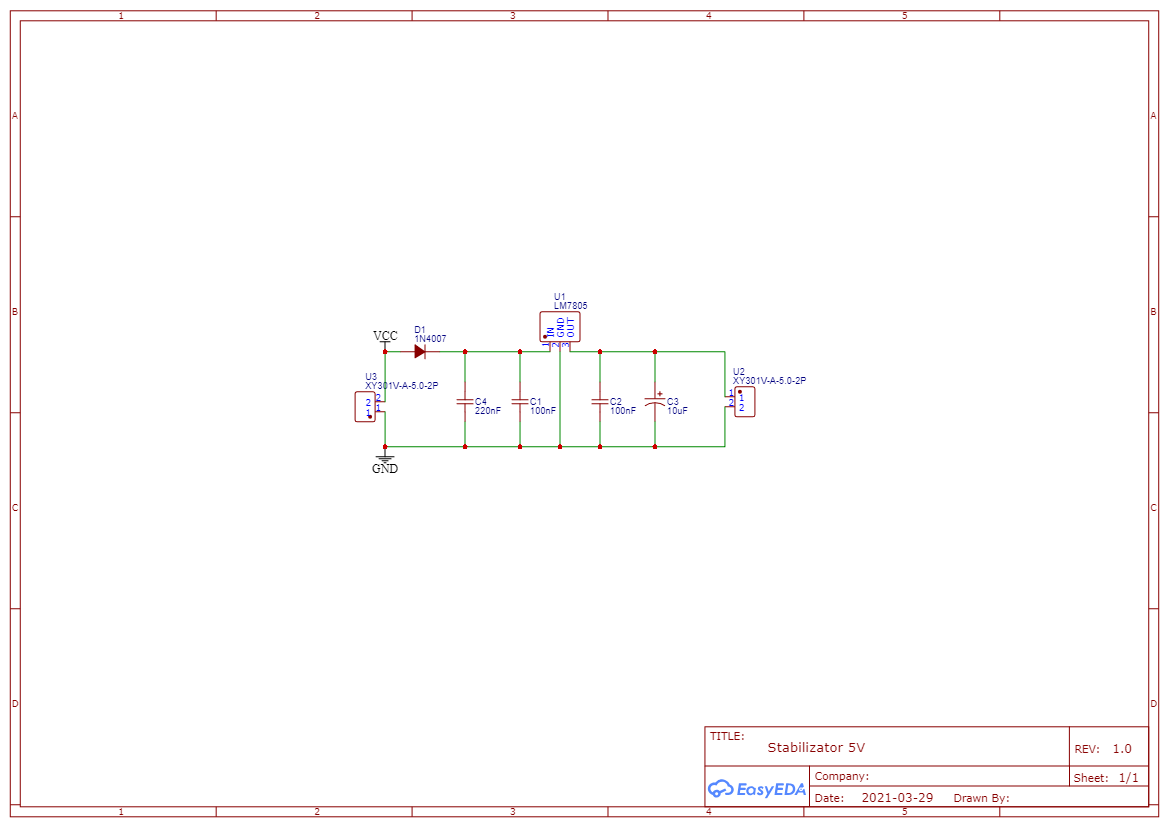
\includegraphics[width=1.0\linewidth]{schemat_stabilizator}
			\caption{Schemat stabilizatora napięcia}
			\label{fig:schematstabilizator}
		\end{figure}\\
		\subsubsection{Widok PCB}
		Zastosowanie montażu przewlekanego pozwoliło w łatwy sposób wykonać płytkę w warunkach domowych.
		\begin{figure}[H]
			\centering
			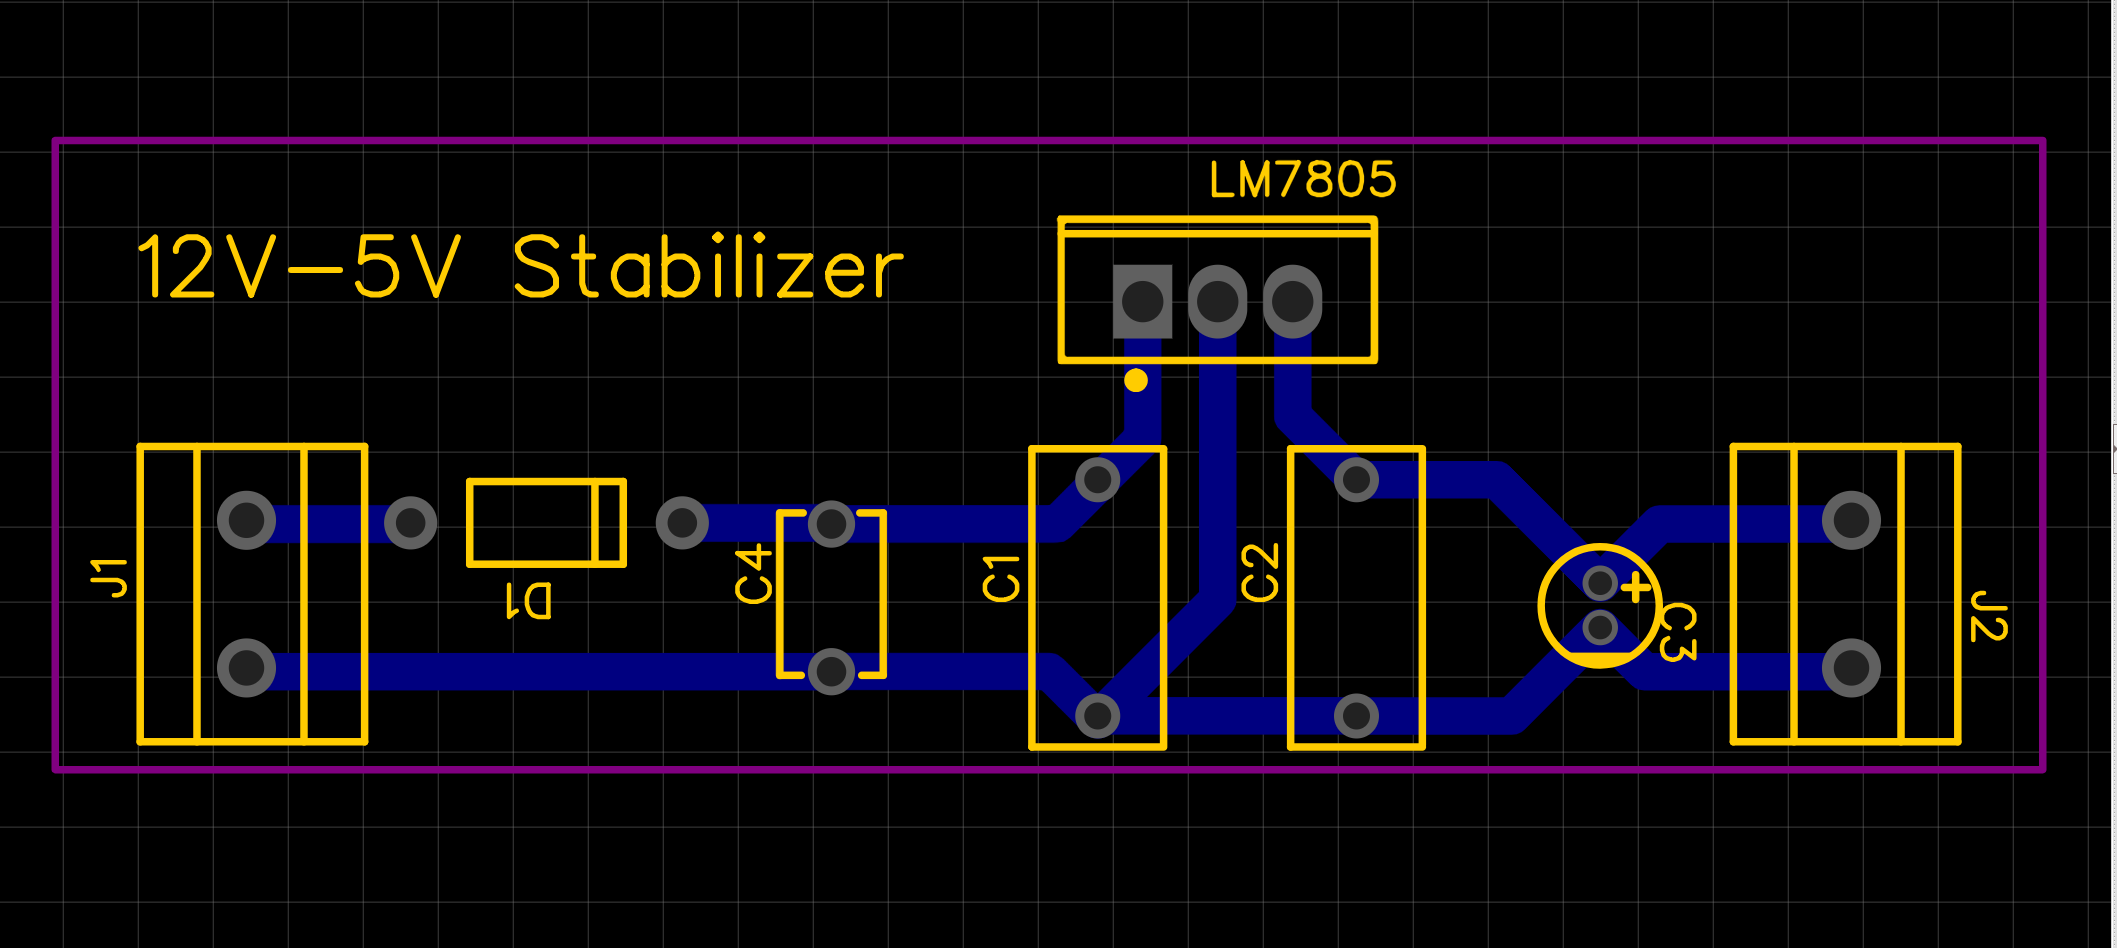
\includegraphics[width=0.7\linewidth]{stabilizator_PCB}
			\caption{Widok PCB stabilizatora w programie EasyEDA}
			\label{fig:stabilizatorpcb}
		\end{figure}
		\subsubsection{Produkcja PCB}
		Ścieżki, wydrukowane laserowo, przeniesiono na miedź metodą transferu acetonowego. Podczas wielokrotnych prób, najlepszym nośnikiem okazały się materiały marketingowe sklepów wielkopowierzchniowych, tzw. gazetki. Wytrawianie przebiegło pod kontrolą czynnika B-327 (nadsiarczanu sodowego). Gotowa płytka pokryta została izopropylowym roztworem kalafonii celem zapobiegania utlenianiu miedzi.
		\begin{figure}
			\centering
			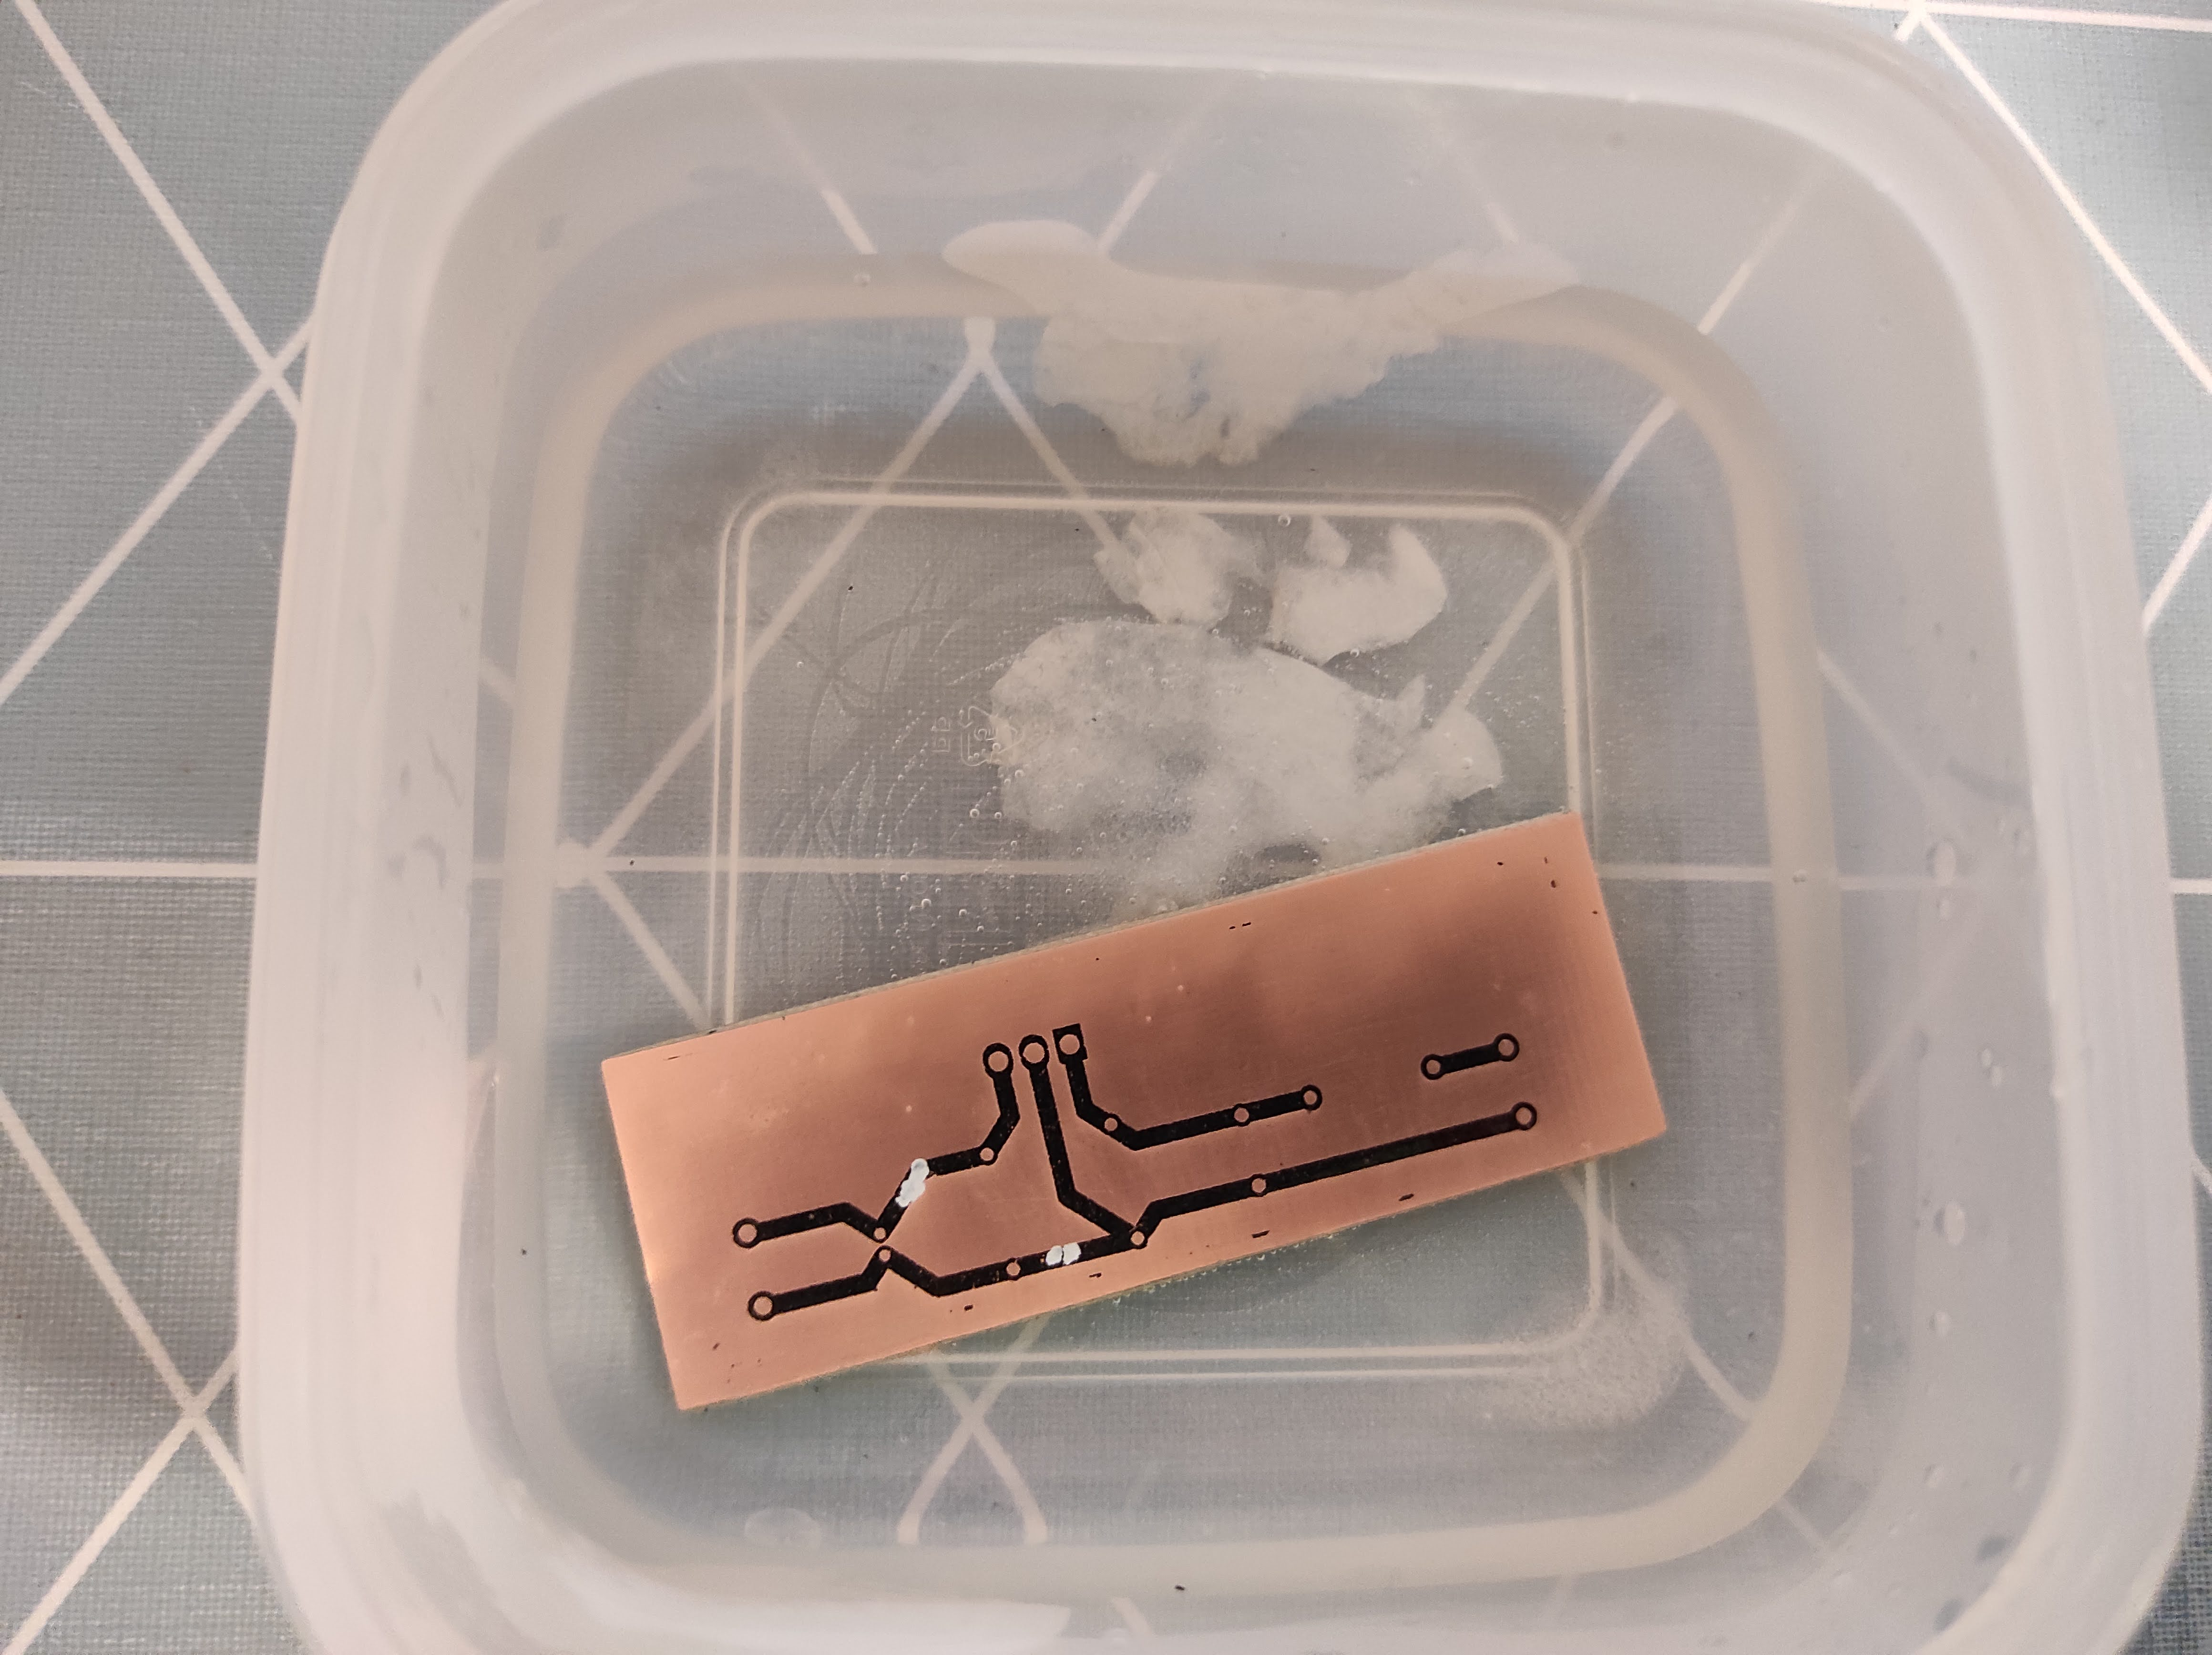
\includegraphics[width=0.7\linewidth]{wytrawianie}
			\caption[Wytrawianie stabilizatora]{Wytrawianie płytki stabilizatora}
			\label{fig:wytrawianie}
		\end{figure}
	
		\begin{figure}
			\centering
			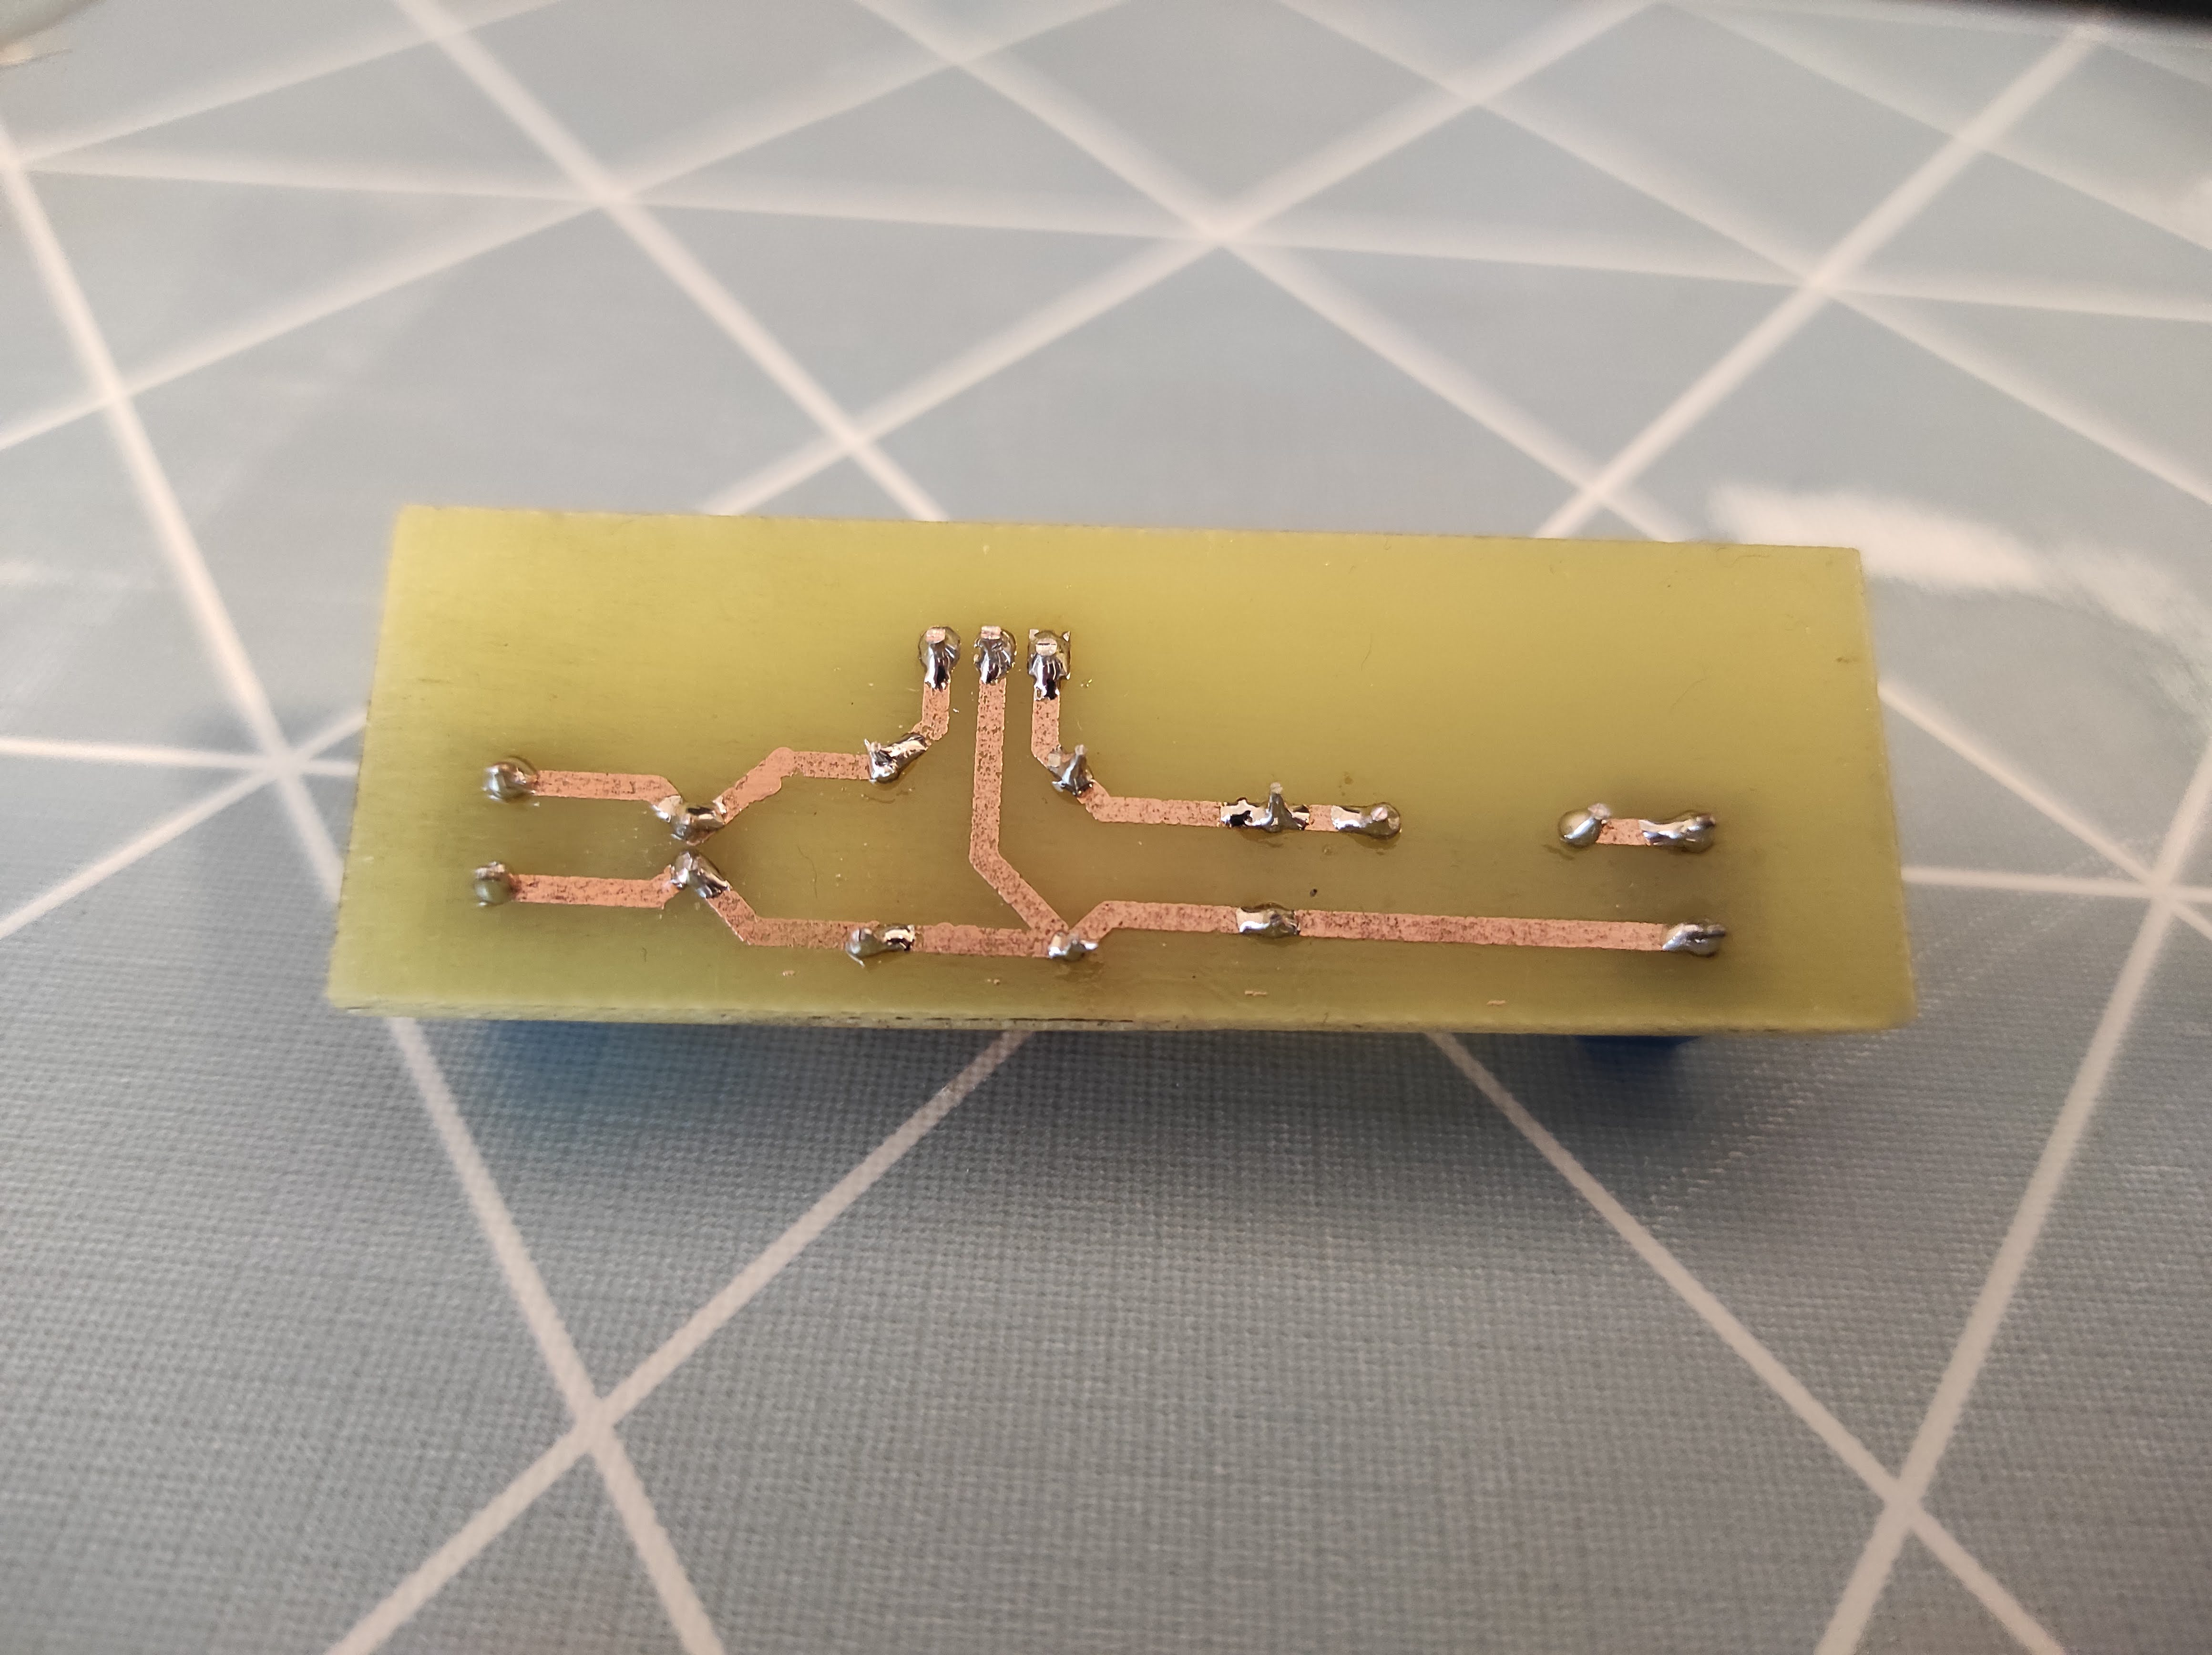
\includegraphics[width=0.7\linewidth]{wytrawione_ścieżki}
			\caption[Wytrawione ścieżki stabilizatora]{Wytrawione ścieżki stabilizatora}
			\label{fig:wytrawionesciezki}
		\end{figure}
		
		\begin{figure}
			\centering
			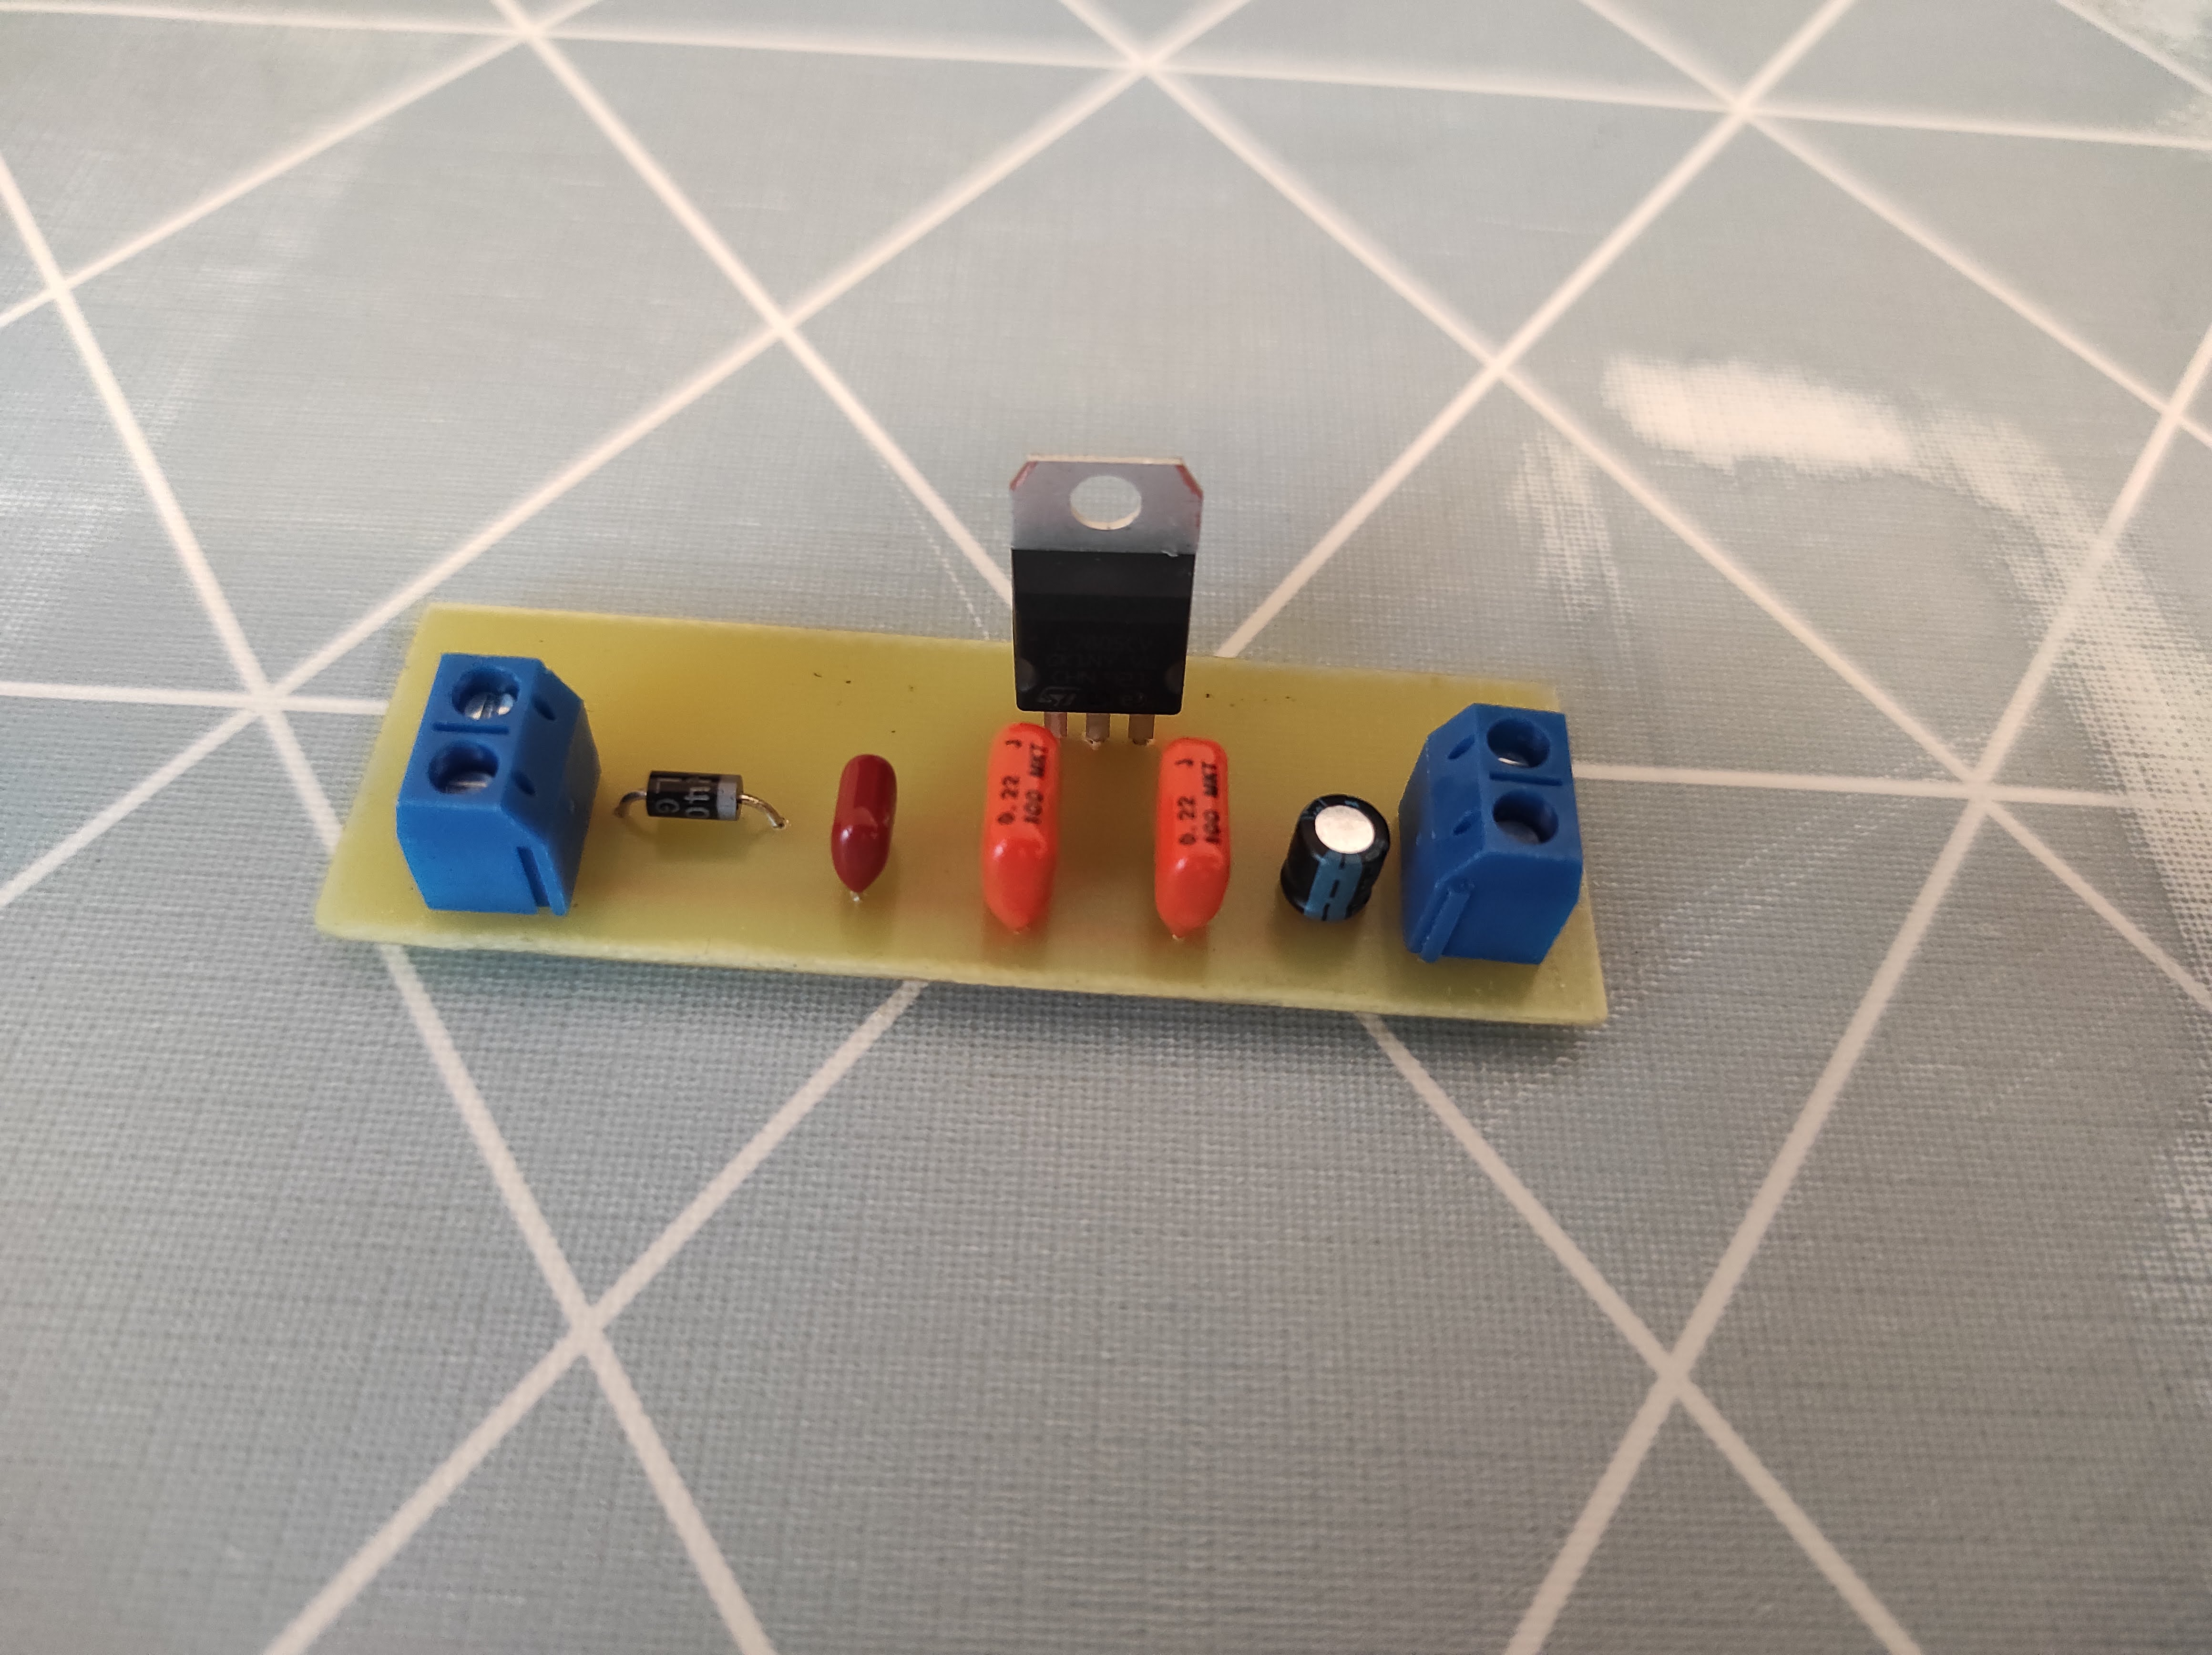
\includegraphics[width=0.7\linewidth]{pcb_gotowe}
			\caption[Zmontowany układ]{Zmontowany układ stabilizatora napięcia}
			\label{fig:pcbgotowe}
		\end{figure}
				\subsubsection{Sprawdzenie poprawności działania}
				Testy układu wykonane multimetrem uniwersalnym pokazały, że po podłączeniu źródła napięcia w postaci akumulatora samochodowego, zarówno z obciążeniem modułami jak i bez niego, układ stabilizatora utrzymuje stałe napięcie bliskie +5V. Układ zatem zadziałał prawidłowo i mógł zostać wykorzystany w projekcie.
		\subsection{Kabel OBD-II}
		Do działania układu niezbędne było wykonanie kabla pozwalającego dostarczyć napięcie oraz sygnały CANH i CANL z gniazda OBD. Kabel wykonano z czterożyłowego przewodu, zakończonego wtykiem męskim OBD. Na zdjęciu widoczne przewody: 
		
		\begin{figure}[H]
			\centering
			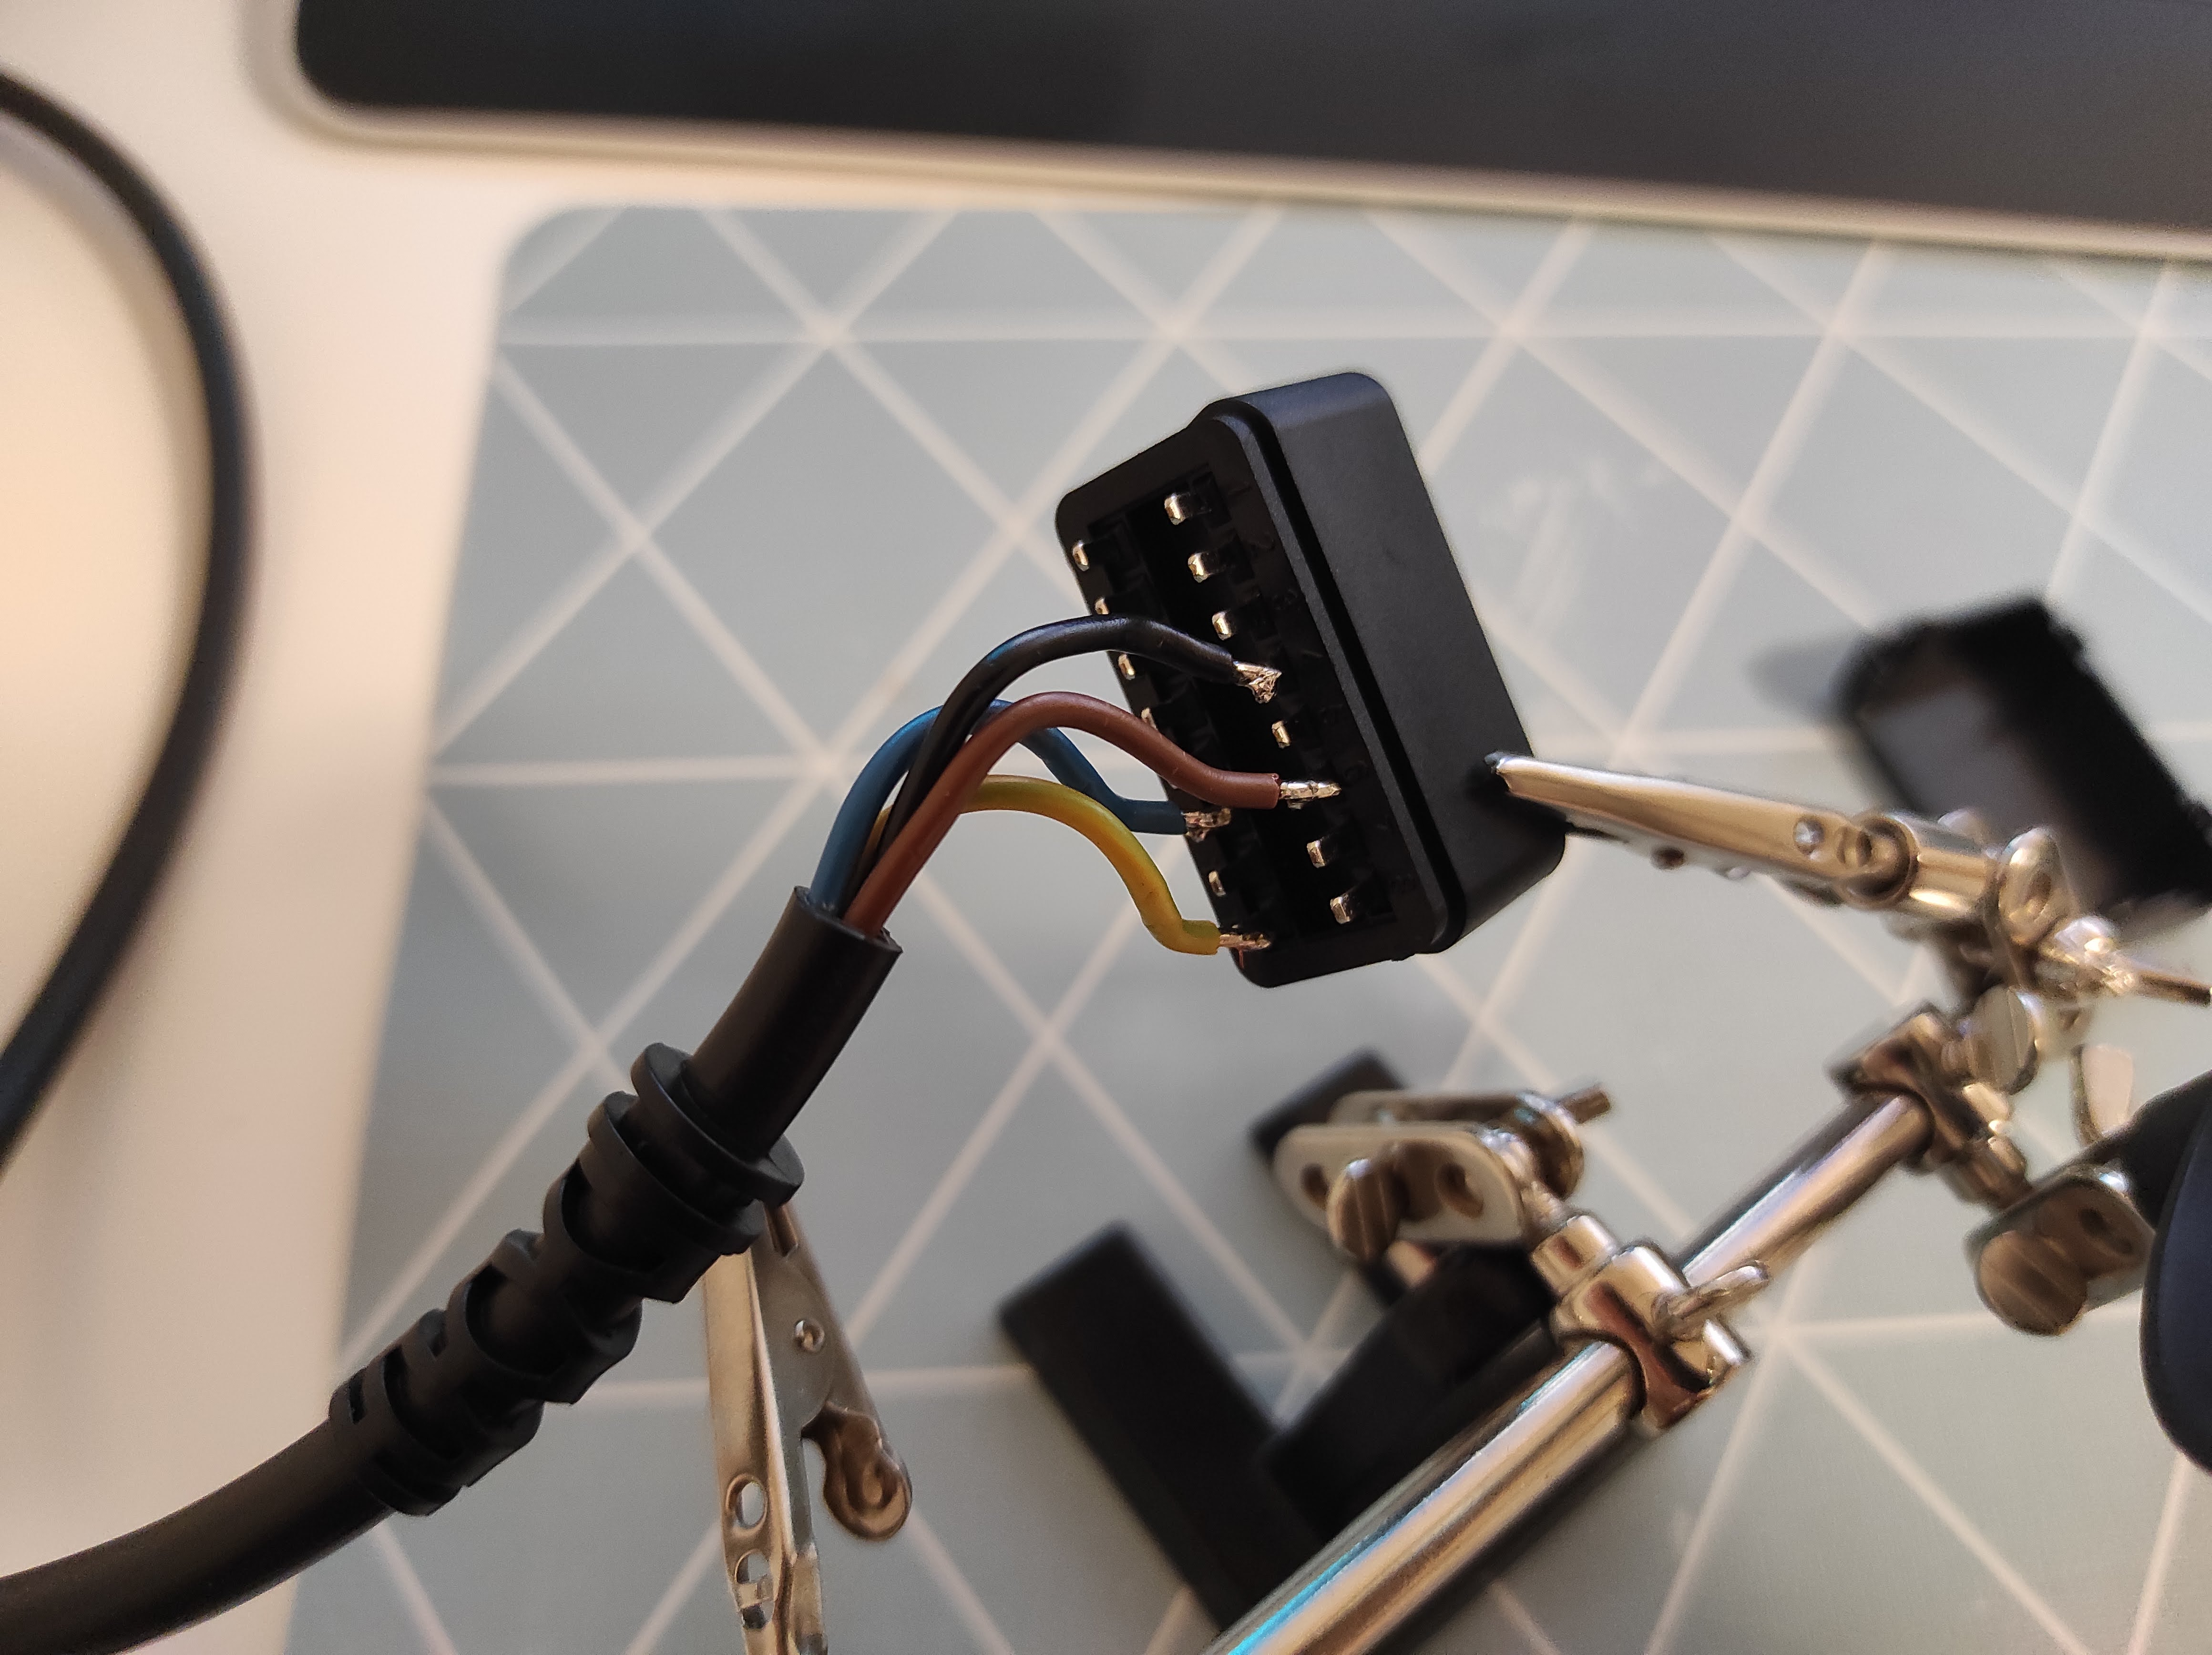
\includegraphics[width=0.7\linewidth]{kabel_obd_2}
			\caption[Kabel z wtyczką OBD-II]{Kabel z wtyczką OBD-II}
			\label{fig:kabelobd2}
		\end{figure}
		
			\begin{table}[H]
			\caption{Kolory przewodów i znaczenie}
			\begin{tabular}{|c|c|c|}
				\hline
				Kolor & Pin & Opis \\
				\hline
				czarny & 4 & masa \\
				\hline
				żółty & 16 & +12V z akumulatora \\
				\hline
				brązowy &6 & CAN High \\			
				\hline
				niebieski &14 & CAN Low \\			
				\hline
			\end{tabular}
		\end{table}
	
	
	\section{Implementacja programowa}
	Programowo, rozwiązanie możemy podzielić na dwie grupy:
		\begin{itemize}
			\item aplikacja działająca po stronie sprzętowej, w samochodzie - VagCan
			\item zestaw aplikacji działających po stronie sieciowej i użytkownika - RemoteCarDiagz
		\end{itemize}
		\subsection{VagCan}
		VagCan napisany jest w języku C++ i działa na platformie NodeMCU.\\
		Do jego zadań należy:
		\begin{itemize}
			\item wysyłanie żądań PID na magistralę CAN
			\item odczyt odpowiedzi z magistrali
			\item wysłanie danych pomiarowych do aplikacji serwerowej z pakietu RemoteCarDiagz
			\item pobieranie aktywnych PID do przeprowadzenia pomiarów z aplikacji serwerowej RemoteCarDiagz
			\item obsługa połączenia WiFi
		\end{itemize}
		\subsubsection {Wykorzystane biblioteki}
		Aplikacja korzysta z kilku bibliotek:
		\begin{itemize}
			\item MCPCAN.h autorstwa Cory J. Fowler - do obsługi protokołu CAN przez MCP2515
			\item ESP8266WiFi.h - obsługa WiFi
			\item ArduinoJson.h - obsługa serializacji i deserializacji danych
		\end{itemize}
		\subsubsection{Algorytm działania}
		Cały program zawarty jest w pliku main.cpp. Z uwagi na prototypowy charakter, a także na niewielki stopień skomplikowania, zaniechano wydzielania poszczególnych metod od osobnych plików. Podobnie jak każdy program na platformie kontrolera NodeMCU, także ten zawiera dwie główne funkcje:
		\begin{itemize}
			\item setup() - uruchamiana tylko raz po resecie mikrokontrolera,
			\item loop() - działająca nieprzerwanie, aż do momentu wyłączenia lub resetu, główna pętla programu
		\end{itemize}
		Przebieg działania metody setup() ilustruje poniższy diagram:
		\begin{figure}[H]
			\centering
			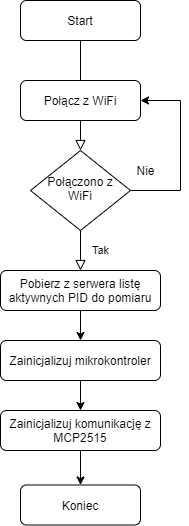
\includegraphics[width=0.2\linewidth]{loop_algorymt}
			\caption[setup()- algorytm działania]{Algorytm działania metody setup()}
			\label{fig:loopalgorymt}
		\end{figure}
		W metodzie loop() działa cała główna logika programu. W ogólności, co 5 sekund wysyłany jest request do aplikacji serwerowej, pobierający aktywne PID, które będą wysyłane w żądaniach diagnostycznych. Odpowiedź z serwera jest deserializowana i zapisywana w tablicy aktywnych PID.
		Co 200 ms wysyłane jest żądanie pomiaru kolejnego aktywnego PID na magistralę CAN. W każdym przebiegu pętli programu sprawdzany jest stan portu GPIO2 mikrokontrolera ESP8266. Stan niski na tymże, oznacza, że w rejestrach MCP2515 są gotowe do odczytu dane diagnostyczne. W takim wypadku, dane zostają odczytane przez ESP8266, zserializowane do postaci JSON i wysłane do aplikacji serwerowej.
		\begin{figure}[H]
			\centering
			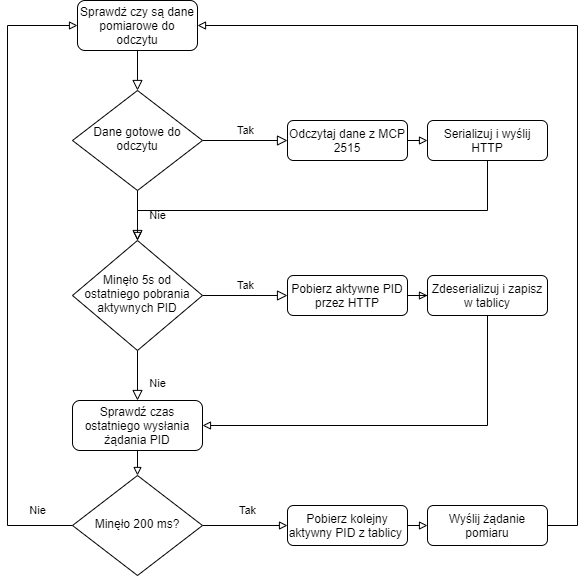
\includegraphics[width=0.5\linewidth]{main_loop.drawio}
			\caption[Algorytm działania metody loop()]{Algorytm działania metody loop()}
			\label{fig:mainloop}
		\end{figure}
		Warto od razu zauważyć wadę takiego rozwiązania. MCP2515 dysponuje dwoma buforami odczytu, działającymi równolegle. Zatem można przekształcić tak działanie programu, aby żądać, odczytywać i wysyłać do serwera dane pomiarowe parami, zamiast pojedynczo. Pozwoliłoby to na pewno bardziej efektywnie wykorzystać czas działania programu, a także zmniejszyć narzut opóźnienia związany ze zbyt częstym wysyłaniem danych przez protokół HTTP.\\
		Kolejną rzucającą się w oczy wadą, jest wpisany w kod programu adres serwera, a także hasło i SSID sieci WiFi. W prototypowym rozwiązaniu jest to dopuszczalne, w przypadku wersji produkcyjnej należy ten problem rozwiązać inaczej- dobrym pomysłem wydaje się dodanie obsługi komunikacji Bluetooth i przesyłanie tych danych w momencie konfiguracji aplikacji poprzez sparowany z mikrokontrolerem telefon. Ciekawym rozwinięciem projektu byłoby dodanie wyświetlacza, lub zestawu LEDów informujących o statusie urządzenia.
		
		\subsection{RemoteCarDiagz}
		Rozwiązanie działające po stronie sieciowej, składa się z kilku serwisów:
		\begin{itemize}
			\item Server - REST API przyjmujące, przetwarzające i zapisujące dane z VagCan oraz GUI; udostępnia dane dla bazy danych Prometheus
			\item Client - GUI - umożliwia użytkownikowi ustawienie aktywnych PID, komunikuje się z Server
			\item aplikacje pomocnicze - baza danych pomiarowych Prometheus oraz Grafana odpowiedzialna za ich wizualizację
		\end{itemize}
		\begin{figure}[H]
			\centering
			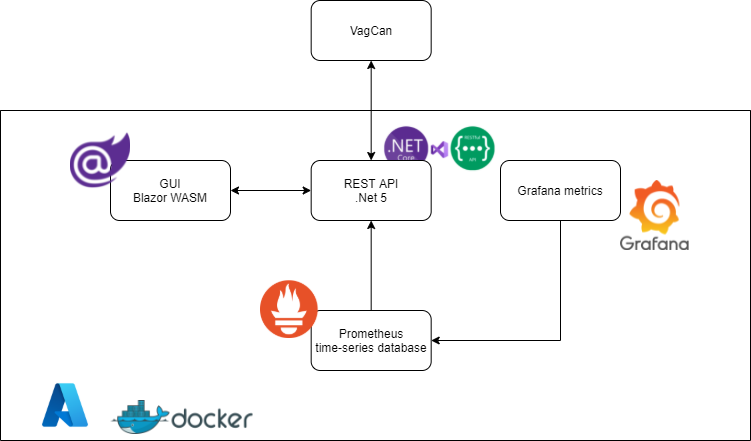
\includegraphics[width=0.8\linewidth]{remoteCarDiagz_schema.drawio}
			\caption[RemoteCarDiagz- schemat ogólny]{RemoteCarDiagz - schemat ogólny}
			\label{fig:remotecardiagzschema}
		\end{figure}
		Całość napisana została w języku C\# dla .Net 5 i umieszczona w pojedynczej solucji. 
		\subsubsection{Server (REST API)}
		Standardowe WEB API, upubliczniające dwa endpointy: /configuration i /measurements a także specjalny, wewnętrzny endpoint /metrics służący do pobierania danych pomiarowych przez aplikację Prometheus.
		\paragraph{\slash configuration} korzysta z niego graficzny interfejs użytkownika (GUI) oraz VagCan. Metoda GET pozwala na pobranie aktualnie aktywnych PID do pomiaru (lub wyświetlenia na GUI), podczas gdy POST zapisuje aktywne PID do bazy danych SQLite.
		\paragraph{\slash measurements} używany jest jedynie przez VagCan - metodą POST przesyłane są wartości pomiarowe, które po obliczeniach trafiają do bazy danych Prometheus
		\subsubsection{Server - przykładowe obliczenia}
		Poniżej pokazano przetwarzanie danych dla PID 0x05, czyli temperatury płynu chłodzącego.
		Dane do serwera trafiają w postaci payloadu JSON:\\
		\begin{lstlisting}
		{
		   "PIDCode": 5,
		   "A": 86,
		   "B": 0,
		   "C": 0,
		   "D": 0
		}
		\end{lstlisting}
		PIDCode jest identyfikatorem PID, natomiast A, B, C, D to wartości poszczególnych bajtów odczytanych przez VagCan z odpowiedzi na żądanie pomiaru PID. Przetwarzanie takiego requestu HTTP polega na przejściu przez łańcuch kolejnych handlerów, z których każdy definiuje sposób wyliczenia odpowiedniej wartości pomiarowej dla danego PID. W przypadku PID 0x05 jest to
		$ A-40 $, zatem zmierzona temperatura płynu chłodzącego wynosi 46 stopni Celsjusza. Tak obliczona wartość jest zapisywana do bazy Prometheus, skąd następnie może zostać zwizualizowana przez Grafanę, w postaci wykresu czasowego.
		\subsubsection{Client - GUI}
		Aplikacja kliencka napisana została z wykorzystaniem frameworka Blazor WASM. Jest to dość szczątkowy interfejs użytkownika, pokazujący jednak możliwość zdalnego sterowania urządzeniem zamontowanym w samochodzie przez stronę www. Dodatkowo, przy wykorzystaniu pakietu Grafana, użytkownik ma możliwość rozbudowanej wizualizacji i analizy danych pomiarowych otrzymanych z pojazdu.
		\begin{figure}[H]
			\centering
			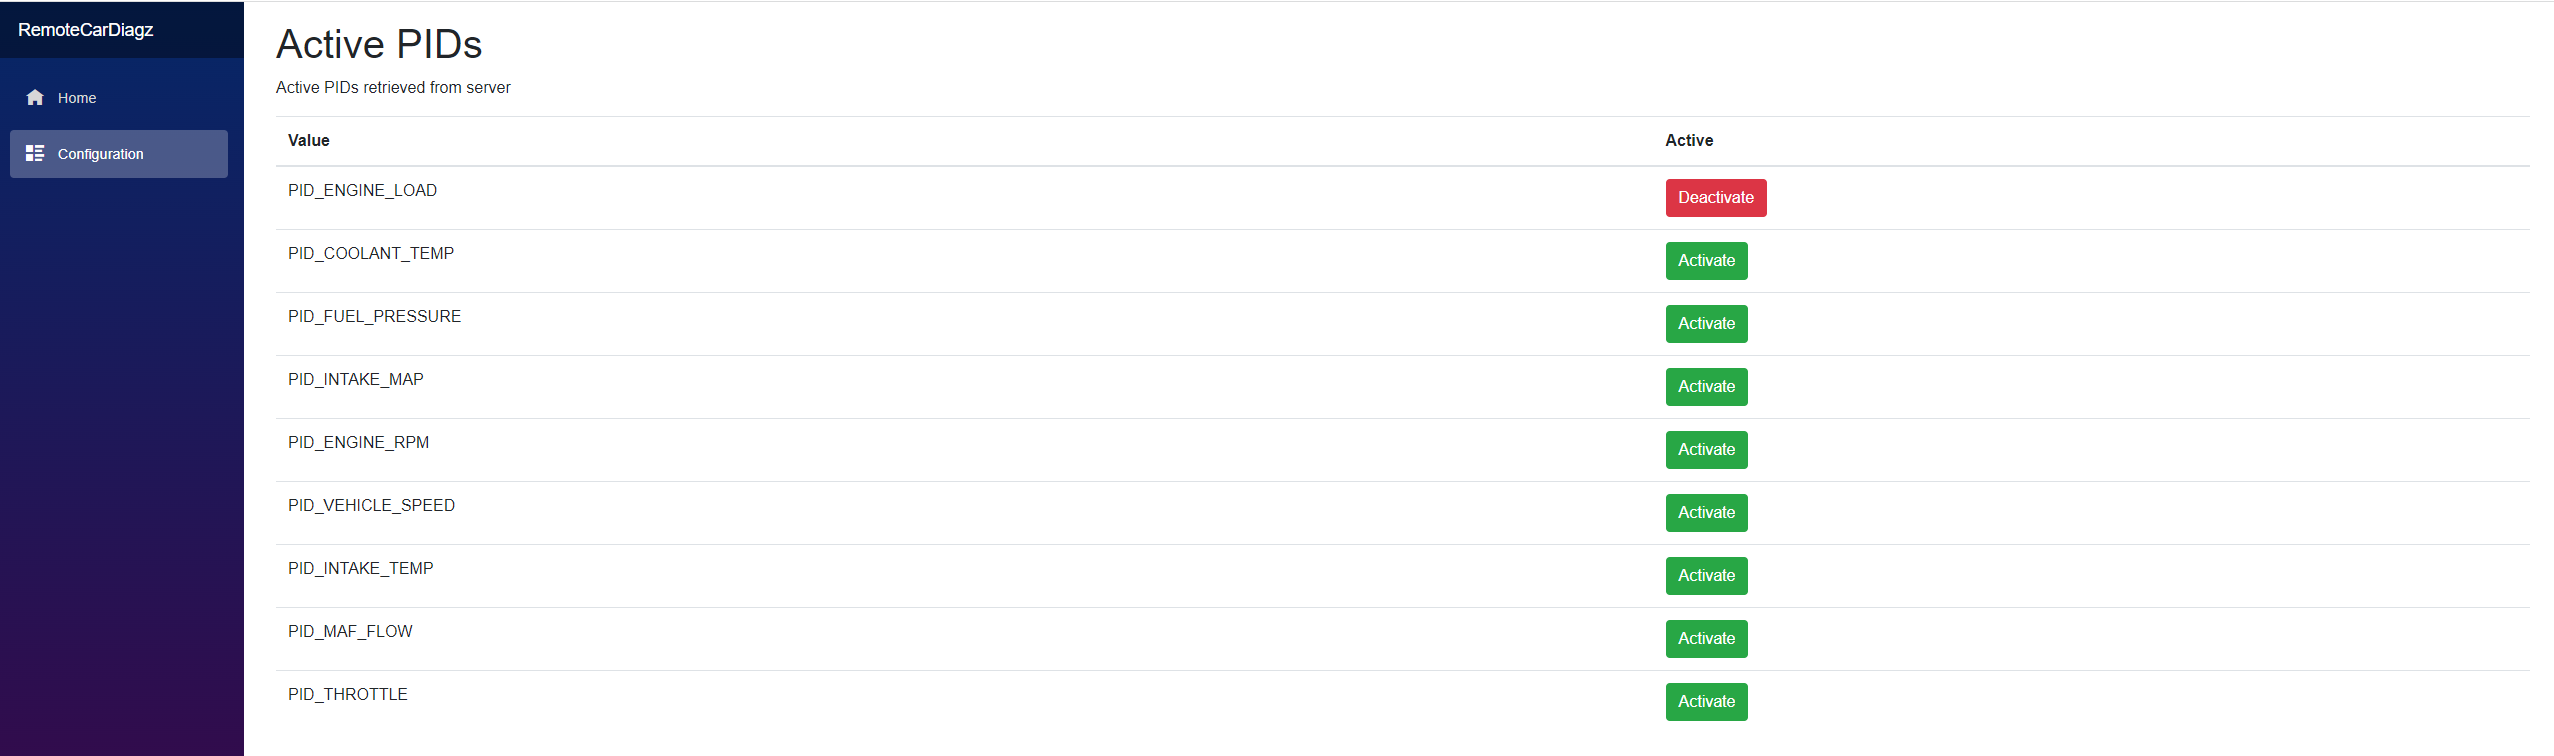
\includegraphics[width=0.9\linewidth]{gui}
			\caption[Zrzut ekranu aplikacji klienckiej]{Zrzut ekranu aplikacji klienckiej - konfiguracja aktywnych pomiarów}
			\label{fig:gui}
		\end{figure}
		Na ekranie widoczna jest lista PID, wspieranych przez aplikację. Spośród wszystkich dostępnych identyfikatorów, zaimplementowano tylko kilka najważniejszych: \\
			\begin{table}[H]
			\caption{Wybrane PID, zaimplementowane w aplikacji}
			\begin{tabular}{|l|l|l|l|}
				\hline
				Nazwa & Kod & Opis & Jednostka \\
				\hline
				PID\textunderscore ENGINE\textunderscore LOAD & 0x04 & Obciążenie silnika & \%  \\
				\hline
				PID\textunderscore COOLANT\textunderscore TEMP & 0x05 & Temperatura czynnika chłodzącego & \degree C \\
				\hline
				PID\textunderscore FUEL\textunderscore PRESSURE & 0x0A & Ciśnienie paliwa & kPa \\
				\hline
				PID\textunderscore INTAKE\textunderscore MAP & 0x0A & Ciśnienie bezwzględne w kolektorze dolotowym & kPa \\
				\hline
				PID\textunderscore ENGINE\textunderscore RPM & 0x0B & Obroty silnika & RPM\\
				\hline
				PID\textunderscore VEHICLE\textunderscore SPEED & 0x0D & Prędkość samochodu & km\slash h\\	
				\hline
				PID\textunderscore INTAKE\textunderscore TEMP & 0x0F & Temperatura powietrza w kolektorze dolotowym & \degree C\\
				\hline
				PID\textunderscore MAF\textunderscore FLOW & 0x10 & Przepływ w czujniku masowego przepływu powietrza & grams/sec \\
				\hline
				PID\textunderscore THROTTLE & 0x10 & Stopień otwarcia przepustnicy & \% \\		
				\hline
			\end{tabular}
		\end{table}
	
		Interfejs użytkownika pozwala na zmianę stanu danego identyfikatora. Stan aktywny oznacza, że identyfikator będzie cyklicznie wysyłany na magistralę CAN celem zebrania danych pomiarowych wielkości odpowiadających identyfikatorowi. W stanie nieaktywnym, nie będą zbierane dane pomiarowe tego identyfikatora.\\		
		W projekcie, po stronie serwera, wykorzystano dwa serwisy pomocnicze - Prometheus i Grafana.
		
		\subsubsection{Prometheus}
		Prometheus jest zestawem narzędzi służącym do monitorowania aplikacji, powstałym w 2012 roku w firmie SoundCloud. Jego głównym zadaniem jest zbieranie i składowanie różnego rodzaju metryk. W uproszczeniu, metryka to para klucz - wartość wraz ze znakiem czasowym (timestamp). W przypadku tego projektu, taką metryką jest para PID - wartość, zarejestrowana w danym czasie. Użycie tego pakietu pozwoliło pominąć implementację bazy danych dla wyników pomiarów, co za pewne byłoby dużo mniej efektywne od wbudowanej w pakiet. Ponadto, ten zestaw narzędziowy doskonale współpracuje z Grafaną, dla której jest domyślnym konfigurowalnym źródłem danych.\\
		Prometheus, co 500 ms pobiera zapisane w pamięci aplikacji Server metryki i kolekcjonuje je w swojej bazie danych. Dodanie do projektu jego obsługi, sprowadza się do zainstalowania pakietu NuGet i odpowiedniej, kilkulinijkowej konfiguracji w kodzie źródłowym.
		
		\subsubsection{Grafana}
		Wizualizacja danych pomiarowych zrealizowana została przy pomocy systemu wspomagającego Grafana. Jest to system szeroko używany w aplikacjach sieciowych, służący do obrazowania danych uszeregowanych czasowo. Użytkownik końcowy ma możliwość wglądu zarówno w chwilowe wartości danych diagnostycznych, jak i przeglądanie ich w wymiarze czasowym, w postaci wykresów. Interfejs umożliwia operacje związane z analizą danych (np. obliczanie średniej lub maksymalnej wartości w czasie) a także operacje graficzne, m.in. powiększanie wykresu, czy wybór przedziału czasowego analizy danych. Źródłem danych jest Prometheus, odpytywany periodycznie co 500 ms.
		
		\subsubsection{Hosting}
		Każdy z wymienionych komponentów, tj. Client, Server, Grafana i Prometheus jest hostowany jako grupa kontenerów Docker w chmurze Azure. Ponieważ kontenery w grupie działają w jednej podsieci, niezwykle łatwo nawiązać między nimi łączność. Ponadto deployment całej grupy kontenerów jest bardzo prosty, sprowadza się do wykonania kilku poleceń w linii komend Azure (Azure CLI). Warto zauważyć, że aplikacja kliencka, jako statycznie kompilowana strona www, nie może być bezpośrednio hostowana z systemu Docker - dlatego dodatkowo wbudowano w kontener serwer Nginx w trybie reverse - proxy. Z uwagi na ograniczoną ilość środków do wykorzystania na platformie Azure przy subskrypcji studenckiej, nie zaimplementowano statycznego adresu IP, w związku z czym po każdym deploymencie adres ten jest inny. Rozwiązaniem tego problemu w środowisku produkcyjnym byłoby zastosowanie Azure Gateway, czyli bramy stojącej przed całą grupą kontenerów i odpowiednio przekierowującej ruch, a także zapewniającej pożądany, statyczny adres IP.
		
		\section{Praca zespołowa}
		Niemożność znalezienia zespołu projektowego spowodowała, że zadanie zostało wykonane samodzielnie. Z uwagi jednak na cel przedmiotu, prace projektowe prowadzone jednak były tak, aby łatwo dały zaadaptować się do większej liczby uczestników projektu.
		
		\subsection{Metodologia}
		Jako metodologię pracy przyjęto model Agile/Scrum. Okres pracy projektowej został podzielony na tygodniowe sprinty. Zadania zostały rozpisane na początku pracy (backlog) oraz został stworzony harmonogram. 
		W rzeczywistym projekcie zespołowym, miałby zastosowanie pełen ceremoniał Scrum, tzn:
		\begin{itemize}
			\item codzienne, krótkie spotkania zespołowe organizujące pracę (maksymalnie 15 minutowy stand-up)
			\item po zakończeniu każdego sprintu demonstracja jego osiągnięć (czyli np. prezentacja działającego oprogramowania lub jego części)
			\item również po zakończeniu sprintu spotkanie retrospektywne (co poszło dobrze, co gorzej, jak możemy to poprawić)
			\item analiza zadań, tak aby każdy członek zespołu miał wiedzę potrzebną do ich wykonania (backlog refinement)
		\end{itemize}
		
		\subsection{Narzędzia}
		Do prowadzenia projektu wykorzystano oprogramowanie Jira. Zadanie projektowe zostało podzielone na Epiki, ukończenie każdego Epiku oznaczało dostarczenie w całości pewnego etapu prac. Każdy z epików dzielony był na user-story, czyli mniejsze zadania, mogące zostać ukończone w kilka do kilkunastu godzin. Poniższy diagram ilustruje ten podział, wraz harmonogramem prac, które jeszcze nie zostały ukończone w danym momencie. Pod nim widoczna jest przykładowa tablica zadań w pojedynczym sprincie, z pokazanym podziałem na zadania w toku, ukończone i nierozpoczęte. Na końcu uwidocznione jest pojedyncze user - story.
				
		\begin{figure}[H]
			\centering
			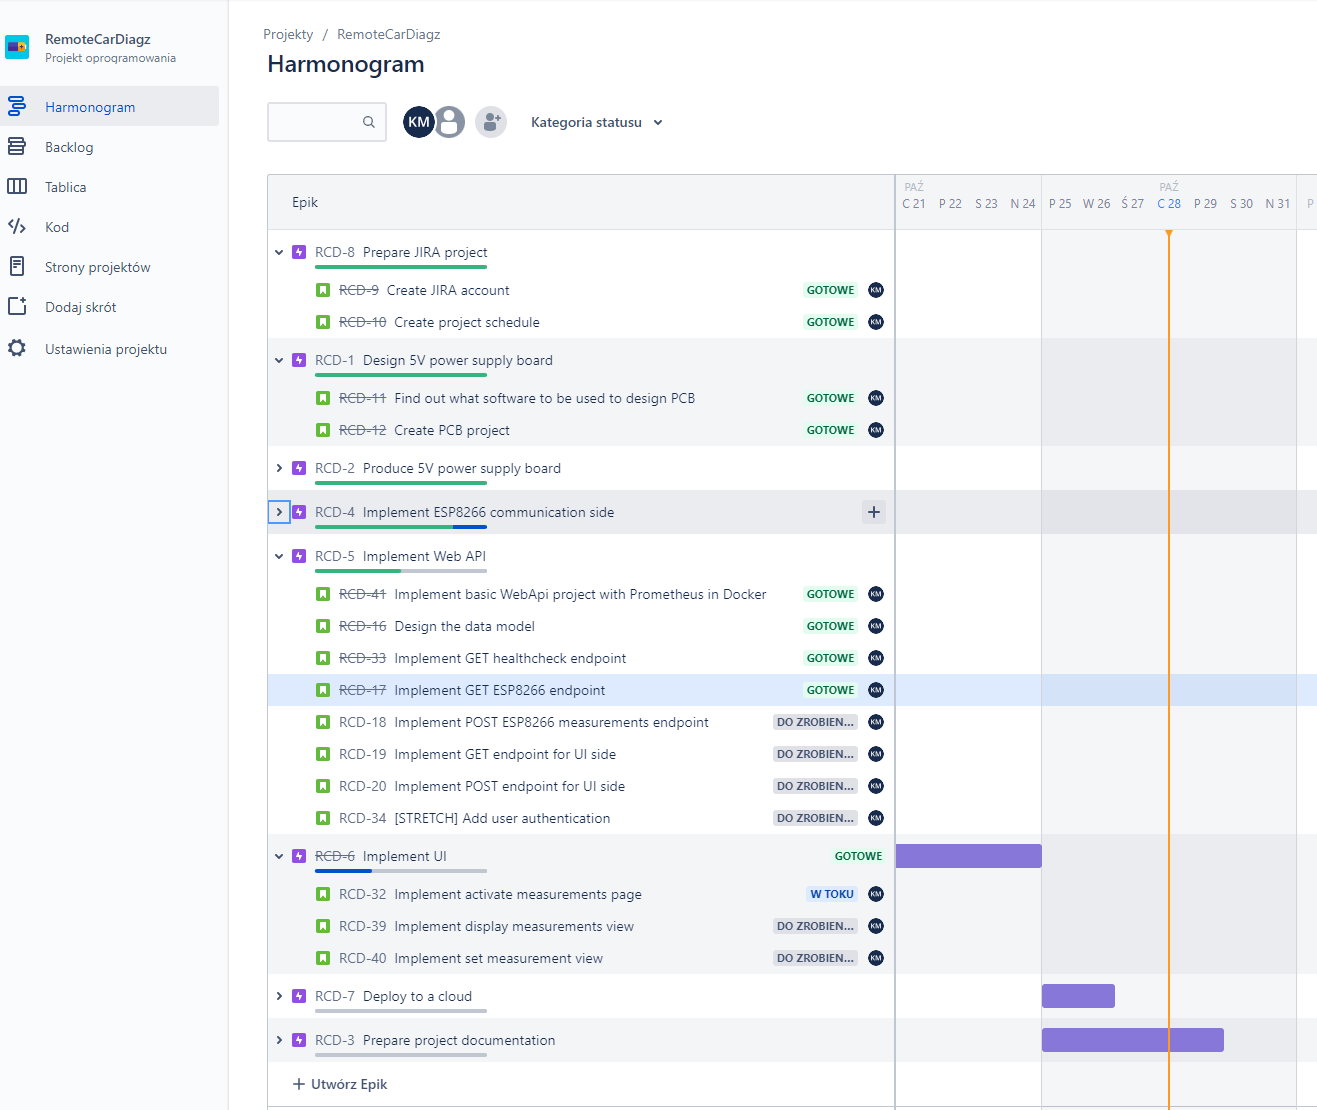
\includegraphics[width=0.9\linewidth]{harmonogram}
			\caption[Harmonogram projektu]{Harmonogram projektu - podział na epiki i user - story}
			\label{fig:harmonogram}
		\end{figure}
		
		\begin{figure}[H]
			\centering
			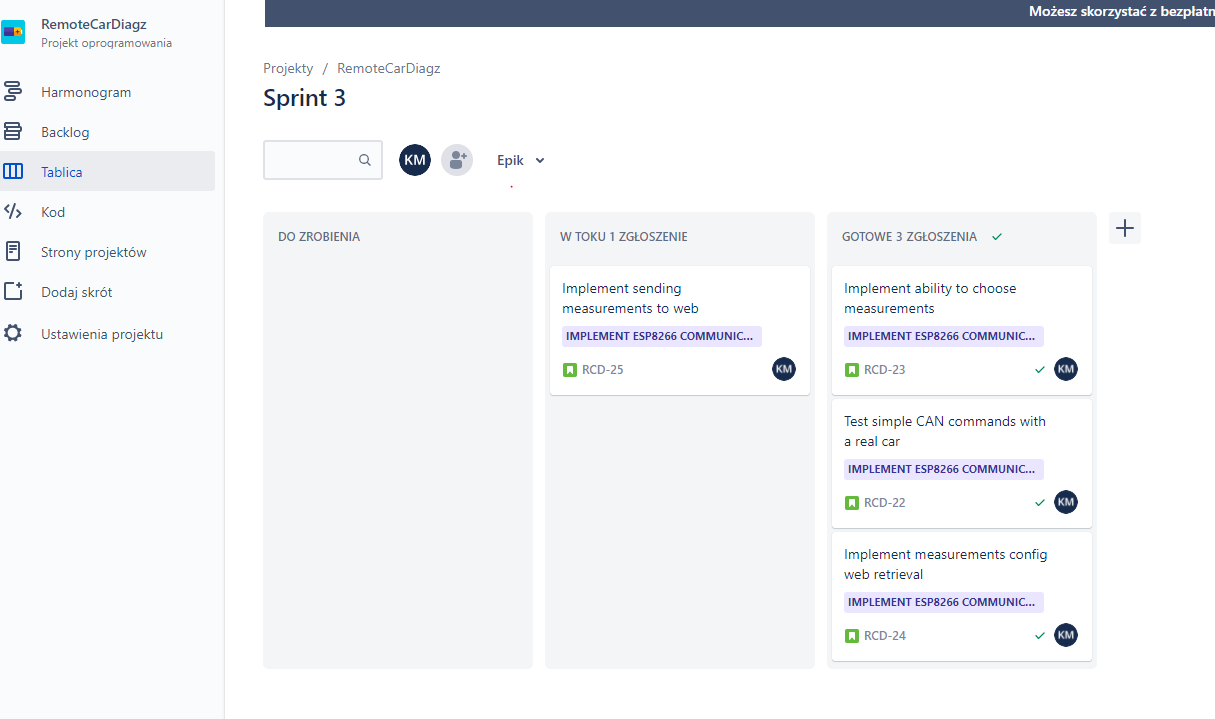
\includegraphics[width=0.9\linewidth]{sprint}
			\caption[Widok tablicy zadań]{Widok tablicy zadań w sprincie}
			\label{fig:sprint}
		\end{figure}
		
		\begin{figure}[H]
			\centering
			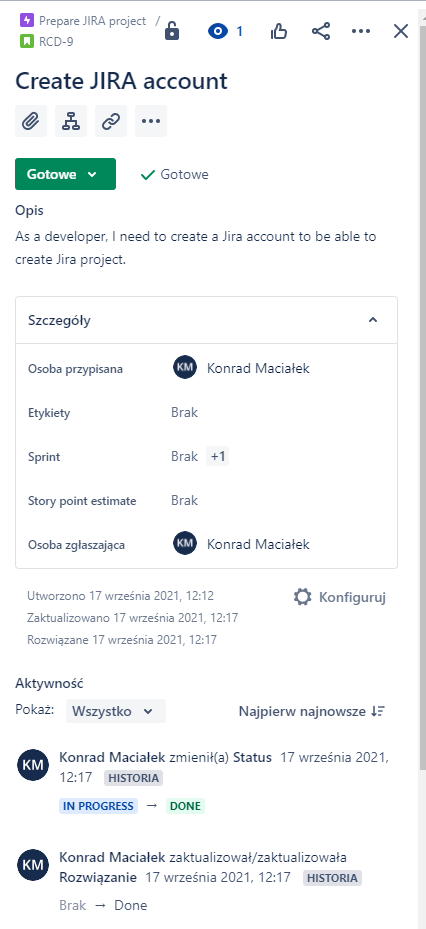
\includegraphics[width=0.5\linewidth]{user_story}
			\caption[User story]{User story}
			\label{fig:userstory}
		\end{figure}
		
		\subsection{Podział zadań w zespole}
		W obranej metodologii pracy oraz dzięki spotkaniom backlog - refinement, każdy członek zespołu powinien być w stanie pracować nad dowolnym user-story widocznym w danym sprincie. Możliwy byłby jednakże również inny podział pracy, np. praca równoległa w dwóch strumieniach - część zespołu zajmuje się stroną sprzętową, druga część - stroną sieciową. W takim przypadku konieczne byłyby spotkania synchronizacyjne, a przede wszystkim odpowiednio wczesne ustalenie kontraktów - interfejsów na granicach domen, którymi zajmowałyby się poszczególne części zespołu.
		
		\section{Podsumowanie}
		\subsection{Efekt prac}
		Efektem prac nad projektem jest powstanie działającego, prototypowego systemu telemetrii samochodowej. Założenia projektowe zostały osiągnięte, działanie zostało przetestowane nie tylko symulacyjnie, ale także w rzeczywistym pojeździe samochodowym. Podczas pracy zapoznano się z nowymi zagadnieniami- przede wszystkim obsługą kontrolera ESP8266, magistrali CAN, czy protokołu OBD. Niezwykle fascynującym procesem było zaprojektowanie oraz własna produkcja płytki PCB stabilizatora napięcia. Także ze strony sieciowej poruszono ciekawe tematy, jak współpraca systemów Prometheus, Grafana z REST API i aplikacją kliencką w kontenerach Docker na platformie Azure. Najwięcej wysiłku pochłonęło pierwsze uruchomienie ESP8266 wraz z MCP2515 i zmuszenie ich do współpracy - okazało się, że winien był nieprawidłowy montaż, przez co obydwa moduły nie miały wspólnej masy, co prowadziło do zupełnie losowych wyników prób ich uruchomienia.
		
		\subsection{Możliwości rozwoju}
		Jak już wielokrotnie wspomniano, jest to układ prototypowy, nie nadający się do zastosowania w środowisku produkcyjnym. Uproszczono wiele procesów, m.in. cała komunikacja odbywa się otwartym protokołem HTTP, zamiast HTTPS, brak jest również jakiejkolwiek autentykacji użytkownika na poziomie interfejsu graficznego klienta, czy podczas wymiany danych między stroną sprzętową a serwerem.\\
		Niemniej jednak, po wyeliminowaniu tych nieprawidłowości, można pokusić się o próby dalszego rozwoju. Przede wszystkim należałoby się skupić na zaprojektowaniu gotowego, zminiaturyzowanego układu, mieszczącego się na jednym PCB, umieszczonym w rozsądnych wymiarów obudowie.
		
		\subsection{Zastosowanie biznesowe}
		Zagadnienie telemetrii jest obecne coraz częściej w naszym życiu. Ilość pojazdów samochodowych zwiększa się rokrocznie, a zbieranie danych diagnostycznych z ich dużej liczby, może dostarczyć ciekawych danych producentom, warsztatom serwisowym, czy właścicielom flot. Koszty prototypu są stosunkowo niskie z powodu wykorzystanych popularnych komponentów, a przy zastosowaniu masowej produkcji stałyby się zapewne jeszcze dużo mniejsze.
		\pagebreak
		\tableofcontents
\end{document}